% main_apsec.tex: APSEC 2026 SEIP paper (<=10 pages incl. appendix + 1 page of refs).
% Scope: the tool IN PRACTICE, evidenced by a two-condition user study.
% The scoring-policy analysis, the verdict-sensitivity bound, the multi-model
% study and the decision study with decision makers belong to a separate
% research paper and must not appear here.
\documentclass[10pt,conference]{IEEEtran}
\IEEEoverridecommandlockouts

\usepackage{cite}
\usepackage{amsmath,amssymb,amsfonts}
\usepackage{graphicx}
\usepackage{booktabs}
\usepackage{tabularx}
\usepackage{array}
\usepackage{microtype}
\usepackage{siunitx}
\usepackage{xcolor}
\usepackage{hyperref}
\usepackage{cleveref}
\definecolor{brandgreen}{HTML}{00915A}
\hypersetup{colorlinks=true,allcolors=brandgreen}
\newcommand{\best}[1]{\textbf{#1}}
\newcommand{\cmark}{\textcolor{brandgreen}{\textbf{Y}}}
\newcommand{\xmark}{\textcolor{black!35}{--}}

\newcolumntype{L}[1]{>{\raggedright\arraybackslash}p{#1}}
\newcommand{\tblsetup}{%
  \footnotesize%
  \setlength{\tabcolsep}{3pt}%
  \renewcommand{\arraystretch}{1.02}%
}

% At most one full-width float at the top of a page: two stacked diagrams
% leave no readable text behind them.
\setcounter{dbltopnumber}{1}

% Tighter float spacing than the IEEEtran defaults (page budget).
\setlength{\textfloatsep}{7pt plus 2pt minus 3pt}
\setlength{\dbltextfloatsep}{7pt plus 2pt minus 3pt}
\setlength{\floatsep}{7pt plus 2pt minus 2pt}
\setlength{\dblfloatsep}{7pt plus 2pt minus 2pt}
\setlength{\abovecaptionskip}{4pt}

% !! Flip to true once data/user_study/{quiz,survey}.csv are collected and
% scripts/analyze_user_study.py --quiz has produced the numbers. The \else
% branch keeps the paper compiling with visible placeholders in the meantime.
\newif\ifstudydone
\studydonetrue
% Filled from `make study-export` output when the flag above is flipped.
\newcommand{\studyN}{eight}
\newcommand{\studyCell}{\textit{--}}
\providecommand{\repourl}{https://github.com/Rqbln/VERA}

\providecommand{\todo}[1]{\textcolor{red}{[TODO: #1]}}
\providecommand{\nax}{\textcolor{black!35}{--}}
\begin{document}

\title{VERA: An Operable Dashboard for Assessing\\ LLM Deployments in Light of the EU AI Act}

% APSEC SEIP is not double-anonymous, so this paper always builds named. The
% block lives in authors_apsec.tex, which is NOT version-controlled: the
% anonymized mirror proxies this repo, so tracked sources carry no identity.
% It is deliberately separate from authors.tex, which serves main.tex (ICSE):
% the two papers do not share an author list.
\author{%
  \InputIfFileExists{authors_apsec}{}{%
    \IEEEauthorblockN{Author list withheld}
    \IEEEauthorblockA{authors\_apsec.tex is absent from this checkout}%
  }%
}

\maketitle

\begin{abstract}
Institutions that deploy large language models in regulated settings must document technical evidence across the six principles the EU AI Act sets out, including environmental impact, before a deployment is approved.
The suites that produce this evidence run from a command line, while the staff who approve deployments work in compliance and risk management and do not write code.
The evidence therefore arrives through an engineer, summarised into a slide and stripped of the detail a reviewer needs to question it.
We present VERA, an open-source self-hosted platform in production in the responsible-AI function of a large European bank.
A reviewer selects a model, runs public benchmarks against it, and reads one score per regulatory requirement, where each score opens onto the tests behind it and each export names the run it came from.
VERA scores the twelve requirements that current benchmarks can measure and adds a thirteenth by instrumenting the energy each evaluation consumes, so environmental impact becomes a measured verdict rather than a written attestation.
Six open-weight models across three families and three sizes exercise all thirteen, and a within-subject study administered by the platform then measures what the presentation changes for a reader.
Across eight participants, correct answers rise from 18 to 32 of 48 and the median time per question falls from 56 to 29 seconds.
The condition order is fixed and the participants are research staff rather than compliance reviewers, so we report an effect on reading rather than on decisions.
VERA and the study instrument are released, so any institution under the same obligation can repeat the measurement on its own deployment, and so the people accountable for an AI release can work from evidence rather than from assurances.
\end{abstract}

\begin{IEEEkeywords}
Responsible AI, EU AI Act, Compliance tooling, User study, Software engineering in practice, Open source
\end{IEEEkeywords}

\section{Introduction}
\label{sec:intro}

Large language models are being built into products across almost every customer-facing function, from answering queries to triaging support requests and drafting documents.
These models are non-deterministic, since their behaviour is learned from the data they are trained on rather than specified by rules, so the same input can produce different outputs across runs.
The same property also leads models to generate confident but false statements, known as hallucinations~\cite{lin2022truthfulqa}, to reproduce text from their training data~\cite{carlini2023extracting}, and to answer the same question differently depending on the social group it names, such as a gender, an ethnicity or a religion~\cite{parrish2022bbq}.
Conventional testing cannot catch behaviour of this kind, since there is no single expected output against which a response can be checked.
Practitioners therefore measure it statistically, over benchmark suites that probe each failure mode~\cite{hendrycks2021mmlu,gehman2020realtoxicity}.

The severity of these failures has led regulators to require such measurement by law rather than leave it to good practice.
The EU AI Act is the most far-reaching of these regulations, and it obliges the provider of a high-risk system to document technical evidence that the system meets a defined set of requirements before it can be deployed~\cite{euaiact2024}.
That evidence must cover the six principles the Act sets out in Recital~27, namely human agency and oversight, technical robustness and safety, privacy and data governance, transparency, diversity and fairness, and social and environmental well-being~\cite{euaiact2024,hleg2019trustworthyai}.
This makes evidence production a routine engineering task that every deployment must complete before it proceeds.

\begin{figure*}[t]
  \centering
  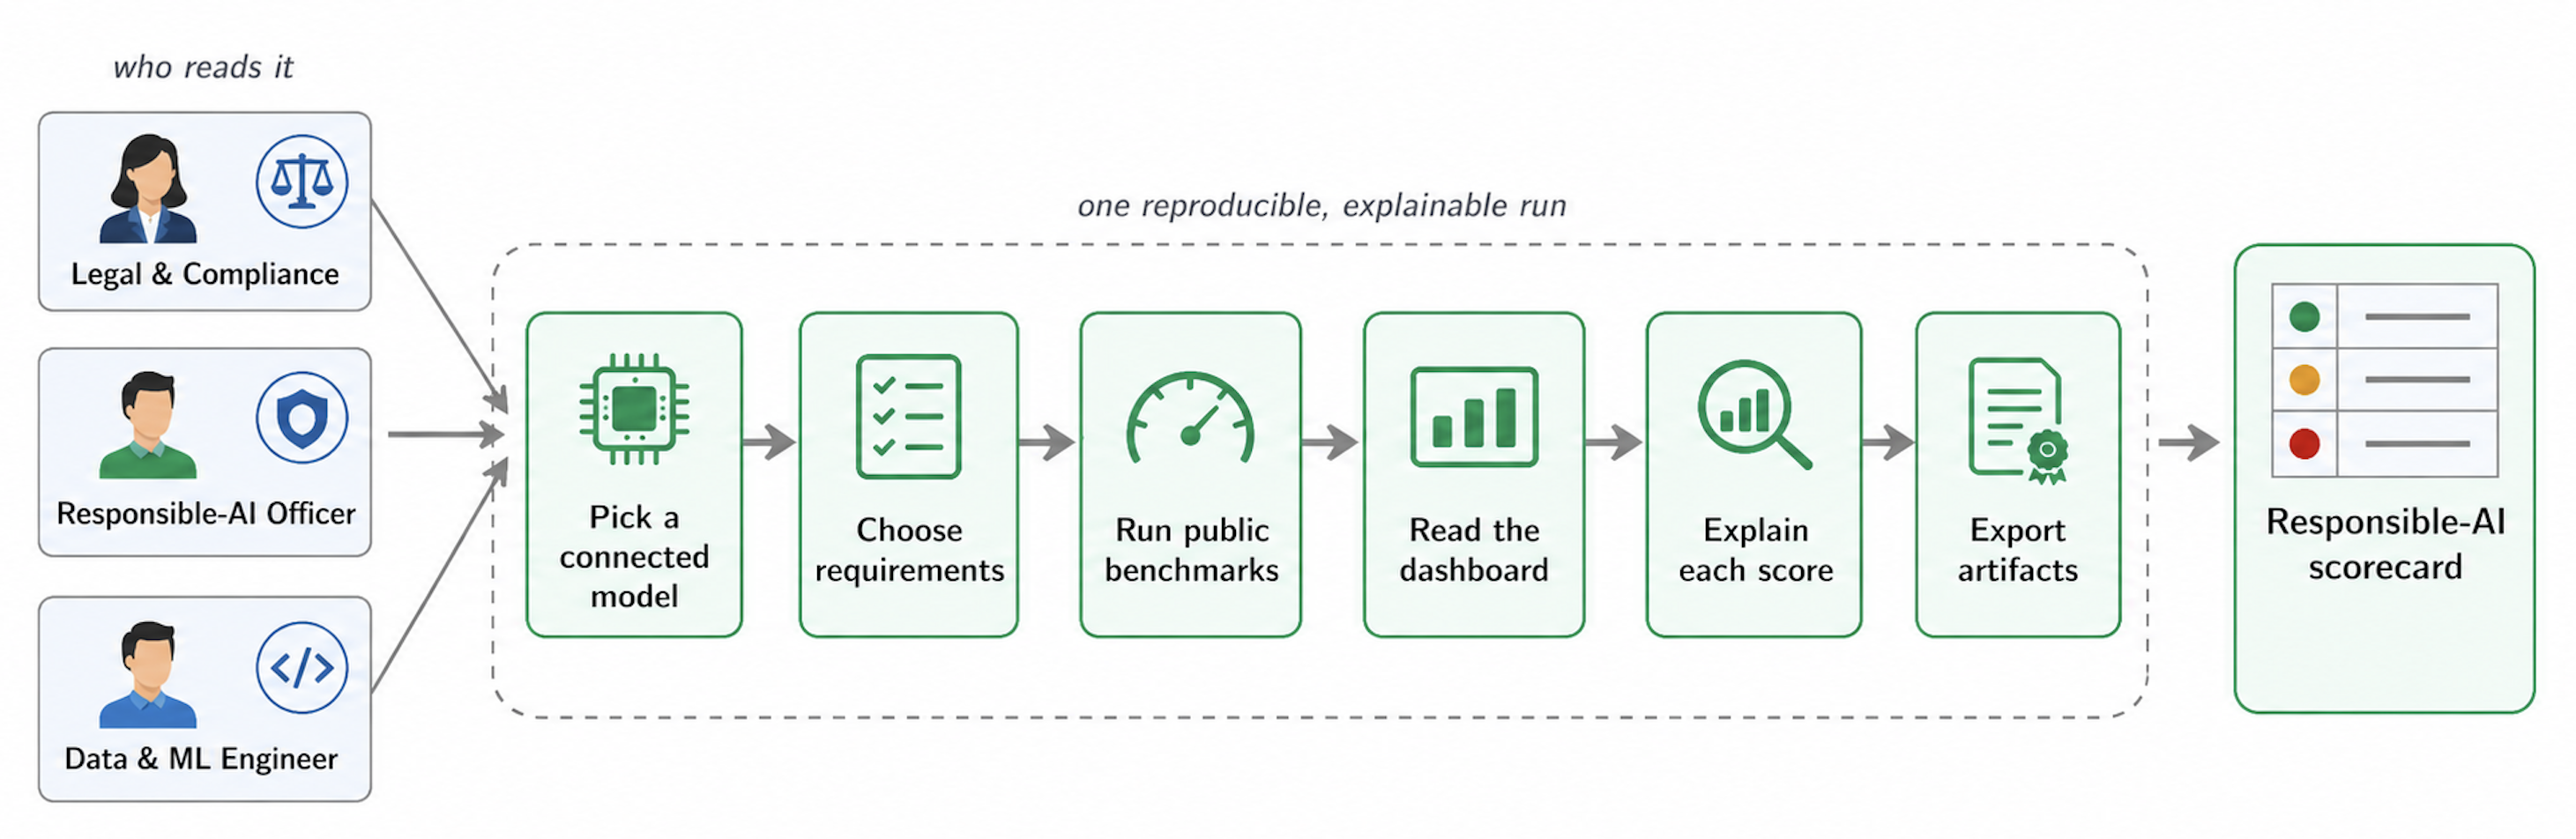
\includegraphics[width=0.80\textwidth]{figures/fig1}
  \caption{The path a user follows, whatever the role. The user selects a served model and a requirement set, runs public benchmarks against it, reads the outcome through a view filtered to that role in which each score can be opened, and exports the evidence tied to that run. 
  % \todo{have we referenced it somewhere?} 
  }
  \label{fig:journey}
\end{figure*}

In a regulated institution, however, the people who produce this evidence and the people accountable for the deployment are not the same.
Approval rests with the second line of defence, in compliance or in risk management, while the evaluation suites are operated by engineers.
Over a year of preparing release decisions in the responsible-AI function of BNP Paribas, we observed three problems that recur because of this separation.
The first is access, since every suite is driven from a command line.
An engineer therefore runs the evaluation and brings a summary slide to the review meeting, where the reviewers cannot interrogate the numbers on it.
The second is opacity, since results arrive as a table of scores with no link to the tests behind them.
A reviewer who asks why a requirement scored poorly must match the run record against per-item outputs by hand.
In one review, a reviewer asked which benchmarks had produced an artificial-intelligence disclosure score of $0.50$ for one model, and answering meant scanning a 209-line harness log to isolate the ten self-disclosure responses behind that requirement, even though every fact needed was already in the files.
The third is drift.
Release documentation is written after the run, so by the time it is filed it describes an evaluation that has already changed.
All three are properties of the software that delivers the measurements rather than of the measurements themselves.

The measurement itself is already well supported.
COMPL-AI maps the Act's principles to eighteen technical requirements and connects twelve of them to public benchmarks~\cite{guldimann2024complai}, while the suites beneath it fix which scenarios a report covers and how each benchmark is executed~\cite{liang2023helm,gao2021lmevalharness,derczynski2024garak,wang2023decodingtrust}.
Run against a served model, these tools write a run record, a harness log and the per-item outputs, which together hold every fact a reviewer needs.
None of them, however, supports reading those files.
Opening them requires a command line, nothing links a requirement score back to the tests that produced it, and the documentation a reviewer takes away does not record which run it came from.
Access, opacity and drift therefore survive a complete measurement, and closing them is the first gap this work addresses.
A second gap lies inside the taxonomy itself, since the remaining six are written up rather than measured, and environmental impact is one of them.
It differs from the other five, because corrigibility and explainability have no agreed technical definition, whereas energy draw is a physical quantity that the Act asks providers to document (Art.~40 Para~2, Annex~XI Para~2e)~\cite{euaiact2024}.
COMPL-AI collects that figure through a form about the resources used in training, although the energy an evaluation itself consumes can be read directly from the host that runs it~\cite{rajput2024fecom}.

To close both gaps, we built VERA (Verifiable Evaluation for Responsible AI), a self-hosted platform that enables a non-specialist to run a requirement-based evaluation of a served model and to read the evidence it produces, from the launch of the run to the filed artifact, and put it into production in the responsible-AI function described above.
A reviewer selects a served model, runs the public benchmark suites against it, and reads a score for each regulatory requirement.
Any score opens onto the benchmarks that produced it and the answers the model gave.
The export that leaves the review names the run behind it, so a later reader can check a figure rather than trust it.
VERA scores all twelve requirements the reference taxonomy can measure, and it adds a thirteenth by instrumenting the energy each evaluation consumes, so environmental impact becomes a measured verdict rather than a written attestation.
Five of the eighteen then remain on a documented human path, rather than six.
\Cref{fig:journey} shows the route a reviewer takes, which needs no account, no configuration file and no code.
A reading layer has to produce output at all before its presentation can matter, so we evaluate VERA on both.
We first run all twelve measurable requirements over six open-weight models, three families at a comparable size and one family at three sizes, which shows that the tool executes the full taxonomy and separates the models it scores.
We then run a within-subject study administered by the platform itself, in which each of eight participants answers six factual questions about one completed evaluation from its raw files and six matched questions on VERA, while the application times each question and validates each answer.
The condition order is fixed and the participants are research staff rather than the compliance reviewers the tool targets, so we report the comparison as an effect on reading rather than on decisions.

This paper makes the following contributions.


\begin{enumerate}
   \item We present VERA, an open-source self-hosted platform that turns a completed evaluation into requirement verdicts a reviewer can read, expand to the tests and model responses behind them, and export with the identity of the run that produced them.
  \item We extend the measurable requirement set from twelve to thirteen by instrumenting the energy each evaluation run consumes, so environmental impact becomes a measured verdict rather than a written attestation.
  \item We provide controlled evidence that presenting an evaluation per regulatory requirement improves the facts a reviewer extracts from it, using a within-subject study that the platform administers.
  \item We identify where that presentation fails, since aggregating benchmarks per requirement hides the coverage a reviewer must count, and a guided launch path does not by itself make a run reachable.
  \item We release the platform, the study instrument that produced these measurements, and the analysis script, available at \url{\repourl}.
\end{enumerate}

% VERA and the study module are available at \url{\repourl}.

% \todo{you dont need this in a 10 page paper.}
% The remainder of this paper is organised as follows.
% \Cref{sec:background} reviews the work on measuring and on reading an evaluation, and states the six requirements.
% \Cref{sec:vera} describes VERA, its six features and its energy instrumentation.
% \Cref{sec:study} gives the evaluation design and \Cref{sec:results} the results.
% \Cref{sec:discussion} interprets those results, \Cref{sec:threats} states what bounds them, \Cref{sec:lessons} reports the deployment experience, and \Cref{sec:conclusion} concludes.


% Résout les numéros de citation sans imprimer la liste (boîte jetée).
\newsavebox\bibbox
\savebox\bibbox{\vbox{\footnotesize\bibliographystyle{IEEEtran}\bibliography{references}}}
\end{document}
